%------------------------------------------------
\section{Results}
%------------------------------------------------
\subsection{Optimal hyperparameters}
\begin{frame}[t]
	\frametitle{Results: Optimal hyperparameters}
	\tikzstyle{background grid}=[draw, black!50,step=.5cm]
	%
	Optimal hyperparameters for the \emph{Seq2Seq} model:\\
	%
	\tikzstyle{background grid}=[draw, black!50,step=.5cm]
	\begin{tikzpicture}[remember picture, overlay] %show background grid, 
		% Put the graphic inside a node. This makes it easy to place the
		% graphic and to draw on top of it. 
		% The above right option is used to place the lower left corner
		% of the image at the (0,0) coordinate. 
		\node [inner sep=0pt,above left, opacity=1.0]  at (1.01\textwidth,-0.73\textheight) (prediction) 
			{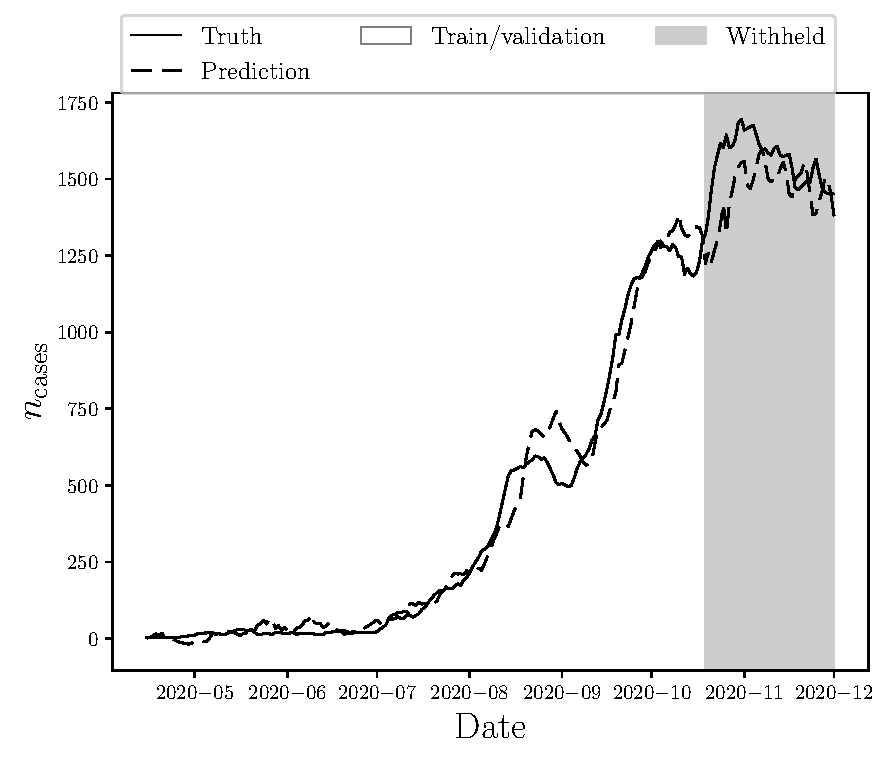
\includegraphics[width=0.5\textwidth]{predictions/model_predictions_test_S2S_mean_Ct_daily_cases.pdf}};
		% show origin
		% \fill (0,0) circle (2pt);
	\end{tikzpicture}%
	%
	\begin{columns}[t] % The "c" option specifies centered vertical alignment while the "t" option is used for top vertical alignment
		\begin{column}{.42\textwidth} % Left column and width
			\vspace{-2.0em}
            % Column widths
            \newcommand{\ocwb}{3.7cm}
            \newcommand{\ocwc}{1cm}
            \newcommand{\ocwd}{1.2cm}
            \newcommand{\ocwe}{3cm}
            %
            \begin{table}[h!]
                \centering
                \footnotesize
                \renewcommand{\arraystretch}{1.5}% Wider
                \begin{tabular}{L{\ocwb}C{\ocwc}C{\ocwd}} \toprule
                    \multicolumn{2}{c}{\bf Hyperparameter}	& \bf Value         \\ \toprule
                    Sliding window size  		& \Ti		&	6				\\
                    Number of hidden neurons	& \nh		&	1500			\\
                    Probability of dropout		& \Pd		&	0.8				\\
                    Number of hidden layers		& \nh		&	2				\\
                    Teacher forcing probability	& \Pt		&	0.3				\\
                    Learning rate 				& \lr		&	$1\times10^{-4}$\\
                    batch size 					& \bs		&	32				\\\hline
                \end{tabular}
            \end{table}
        \end{column}
		%
		\begin{column}{.5\textwidth} % Left column and width
		\end{column}
	
	\end{columns}
	%
	\vspace{-3em}
\end{frame}
%------------------------------------------------
\begin{frame}[t]
	\frametitle{Results: Optimal hyperparameters}
	\tikzstyle{background grid}=[draw, black!50,step=.5cm]
	%
	Optimal hyperparameters for the \emph{support vector machine regression (SVR)} model:\\
	%
	\tikzstyle{background grid}=[draw, black!50,step=.5cm]
	\begin{tikzpicture}[remember picture, overlay] %show background grid, 
		% Put the graphic inside a node. This makes it easy to place the
		% graphic and to draw on top of it. 
		% The above right option is used to place the lower left corner
		% of the image at the (0,0) coordinate. 
		\node [inner sep=0pt,above left, opacity=1.0]  at (1.01\textwidth,-0.73\textheight) (prediction) 
			{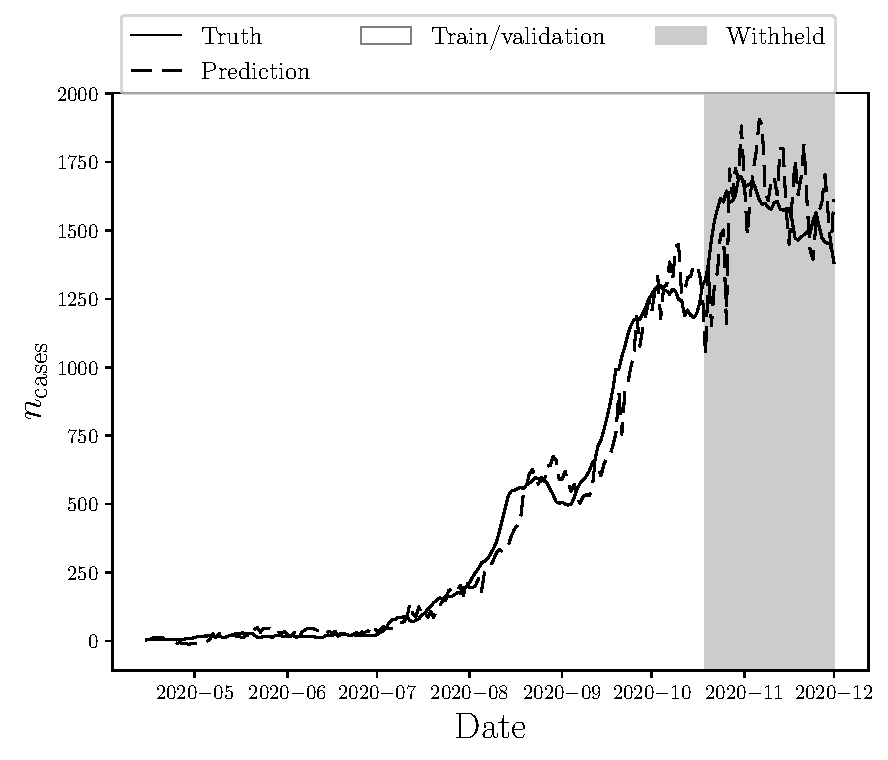
\includegraphics[width=0.5\textwidth]{predictions/model_predictions_test_SVR_mean_Ct_daily_cases.pdf}};
		% show origin
		% \fill (0,0) circle (2pt);
	\end{tikzpicture}%
	%
	\begin{columns}[t] % The "c" option specifies centered vertical alignment while the "t" option is used for top vertical alignment
		\begin{column}{.42\textwidth} % Left column and width
			\vspace{-2.0em}
            % Column widths
            \newcommand{\ocwb}{3.7cm}
            \newcommand{\ocwc}{1cm}
            \newcommand{\ocwd}{1.2cm}
            \newcommand{\ocwe}{3cm}
            %
            \begin{table}[h!]
                \centering
                \footnotesize
                \renewcommand{\arraystretch}{1.5}% Wider
                \begin{tabular}{L{\ocwb}C{\ocwc}C{\ocwd}} \toprule
                    \multicolumn{2}{c}{\bf Hyperparameter}				    & \bf Value             \\ \toprule
                    Sliding window size 						& \Ti	    &	6					\\
                    Ridge factor								& \R	    &	$1\times10^{-4}$	\\
                    Margin of tolerance							& \e	    &	$1\times10^{-2}$	\\
                    Stopping criteria tolerance					& \etol	    &	0.1					\\
                    Learning rate 								& \lr	    &	$1\times10^{-5}$	\\ \hline
                \end{tabular}
            \end{table}
            \uncover<2->{Support vector machine models have \emphasis{deterministic} performance}
        \end{column}
		%
		\begin{column}{.5\textwidth} % Left column and width
		\end{column}
	
	\end{columns}
	%
	\vspace{-3em}
\end{frame}
%------------------------------------------------
\subsection{Prospective validation}
%------------------------------------------------
\begin{frame}[t]
	\frametitle{Results: Prospective validation}
	\tikzstyle{background grid}=[draw, black!50,step=.5cm]
	%
	Performance of models on \emphasis{unseen} data (first 4 months of 2021):\\
	%
	\tikzstyle{background grid}=[draw, black!50,step=.5cm]
	\begin{tikzpicture}[remember picture, overlay] %show background grid, 
		% Put the graphic inside a node. This makes it easy to place the
		% graphic and to draw on top of it. 
		% The above right option is used to place the lower left corner
		% of the image at the (0,0) coordinate. 
		\node [inner sep=0pt,above left, opacity=1.0]  at (1.01\textwidth,-0.73\textheight) (prediction) 
			{
                \only<1>{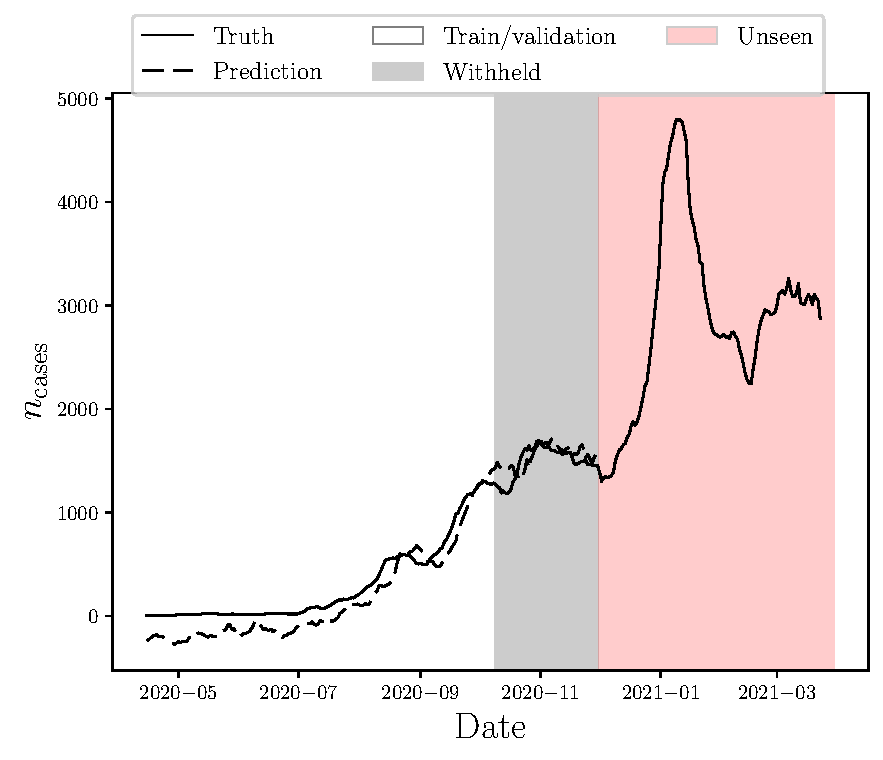
\includegraphics[width=0.5\textwidth]{predictions/model_predictions_unseen_S2S_mean_Ct_daily_cases_truth.pdf}}%
                \only<2>{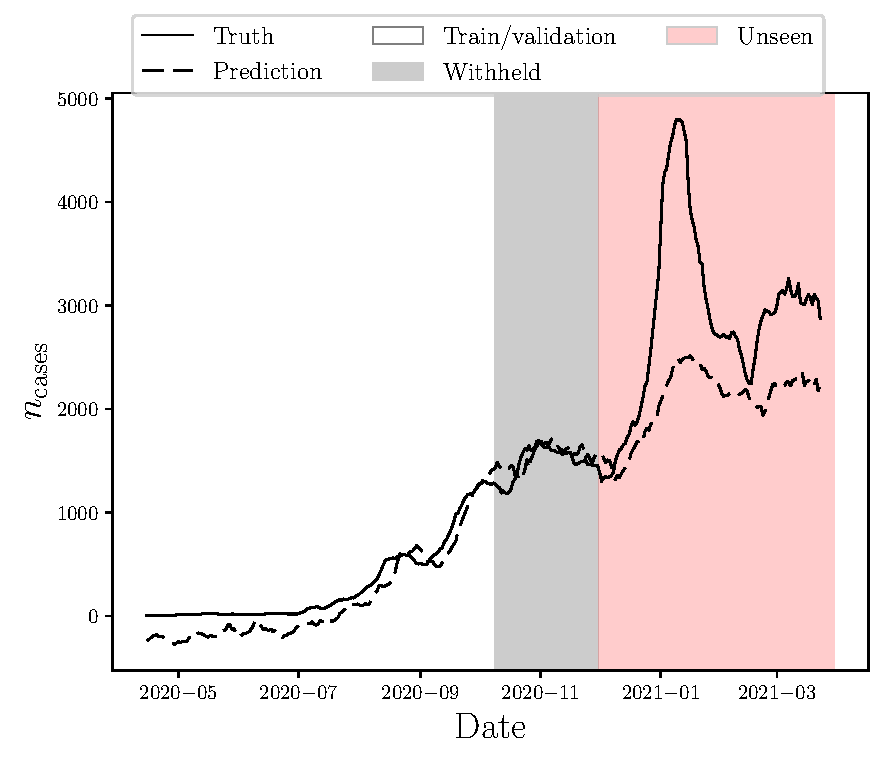
\includegraphics[width=0.5\textwidth]{predictions/model_predictions_unseen_S2S_mean_Ct_daily_cases.pdf}}%
                \only<3>{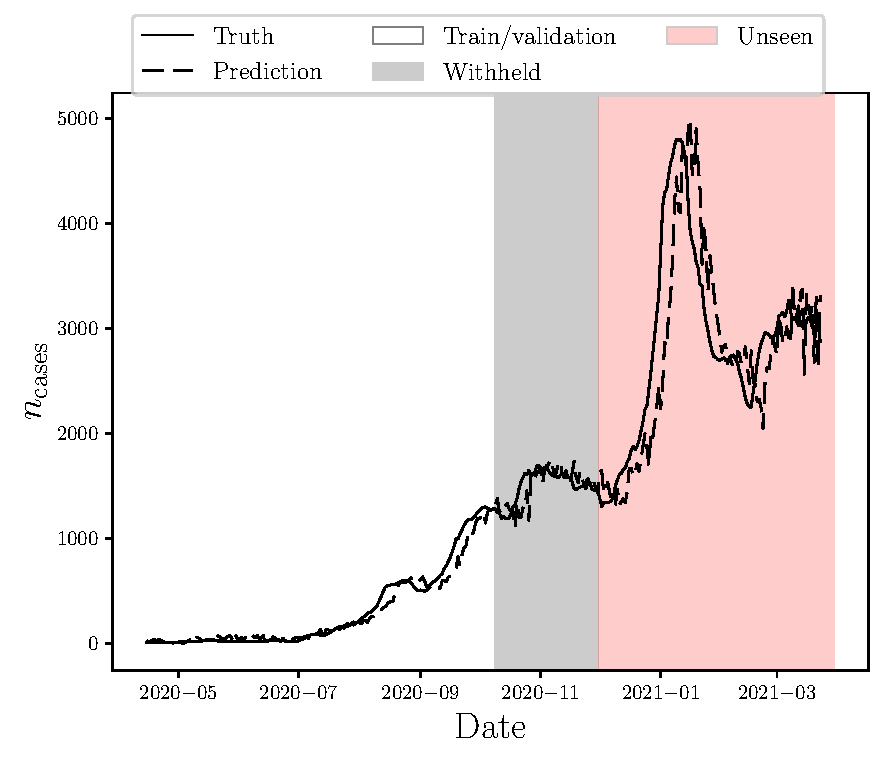
\includegraphics[width=0.5\textwidth]{predictions/model_predictions_unseen_SVR_mean_Ct_daily_cases.pdf}}%
            };
		% show origin
		% \fill (0,0) circle (2pt);
	\end{tikzpicture}%
	%
	\begin{columns}[t] % The "c" option specifies centered vertical alignment while the "t" option is used for top vertical alignment
		\begin{column}{.42\textwidth} % Left column and width
			\vspace{-2.0em}
            % Column widths
            \newcommand{\ocwa}{5cm}
            \newcommand{\ocwb}{1.6cm}
            \newcommand{\ocwc}{1.6cm}
            \newcommand{\ocwd}{1.6cm}
            %
            \begin{table}[h!]
                \centering
                \footnotesize
                \renewcommand{\arraystretch}{1.5}% Wider
                \begin{tabular}{L{\ocwa}C{\ocwd}} \toprule
                    \multicolumn{1}{c}{\bf Model}               & \multicolumn{1}{c}{\bf Test error}    \\ \toprule
                    \only<2>{\emphasis}{Seq2Seq}		        & \only<2>{\emphasis}{0.571}            \\
                    Long short term memory (LSTM) cell          & 0.326                                 \\
                    feedforward neural network	                & 0.255                                 \\
                    \only<3>{\emphasis}{Support vector machine} & \only<3>{\emphasis}{0.168}            \\
                    Gradient boosting 		                    & 1.444                                 \\
                    Linear regression 		                    & 0.160                                 \\ \bottomrule
                \end{tabular}
            \end{table}
        \end{column}
        %
		\begin{column}{.5\textwidth} % Left column and width
		\end{column}
	
	\end{columns}
	%
	\vspace{-3em}
\end{frame}
%------------------------------------------------
\begin{frame}[t]
	\frametitle{Results: Prospective validation}
	\tikzstyle{background grid}=[draw, black!50,step=.5cm]
	%
	Effect of increasing number of training days (Adding 1 month of data):\\
	%
	\tikzstyle{background grid}=[draw, black!50,step=.5cm]
	\begin{tikzpicture}[remember picture, overlay] %show background grid, 
		% Put the graphic inside a node. This makes it easy to place the
		% graphic and to draw on top of it. 
		% The above right option is used to place the lower left corner
		% of the image at the (0,0) coordinate. 
		\node [inner sep=0pt,above left, opacity=1.0]  at (1.01\textwidth,-0.73\textheight) (prediction) 
			{
                \only<1>{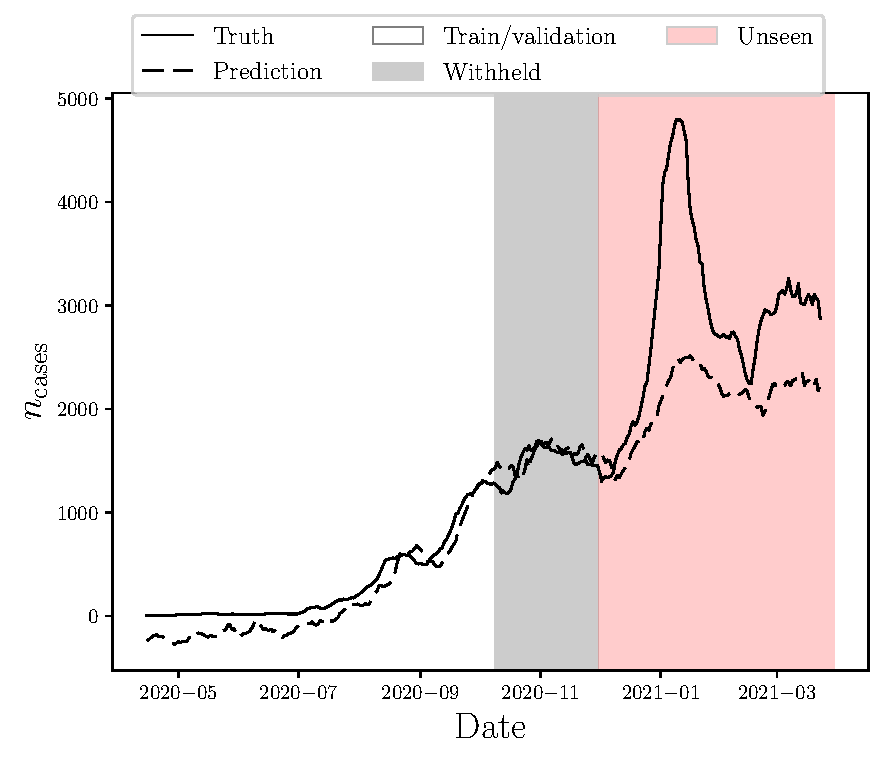
\includegraphics[width=0.5\textwidth]{predictions/model_predictions_unseen_S2S_mean_Ct_daily_cases.pdf}}%
                \only<2>{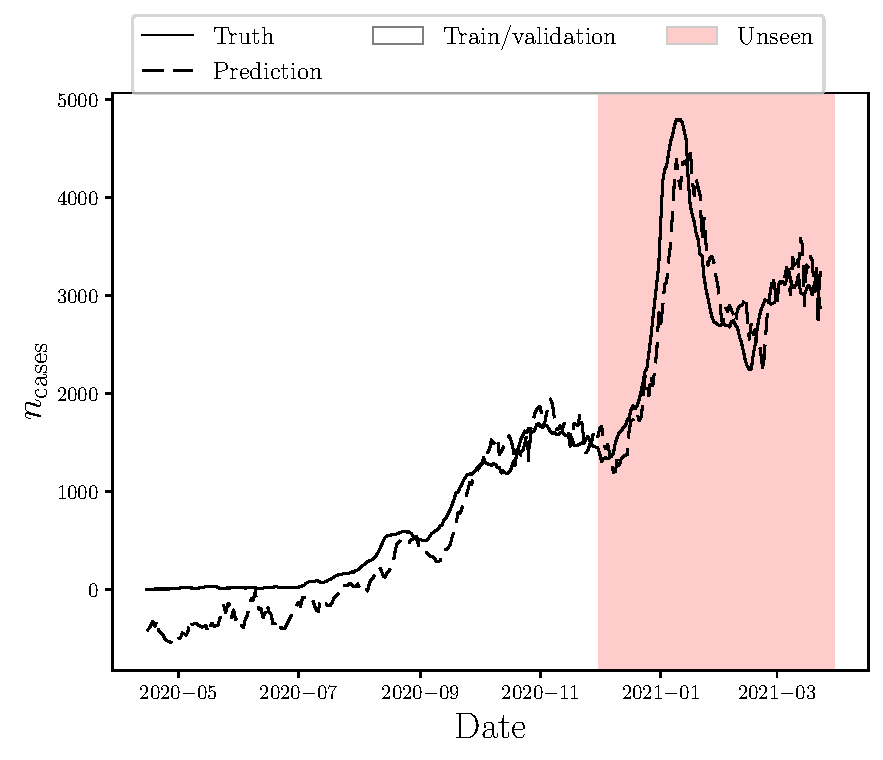
\includegraphics[width=0.5\textwidth]{predictions/model_predictions_unseen_S2S_mean_Ct_daily_cases_G12.pdf}}%
                \only<3>{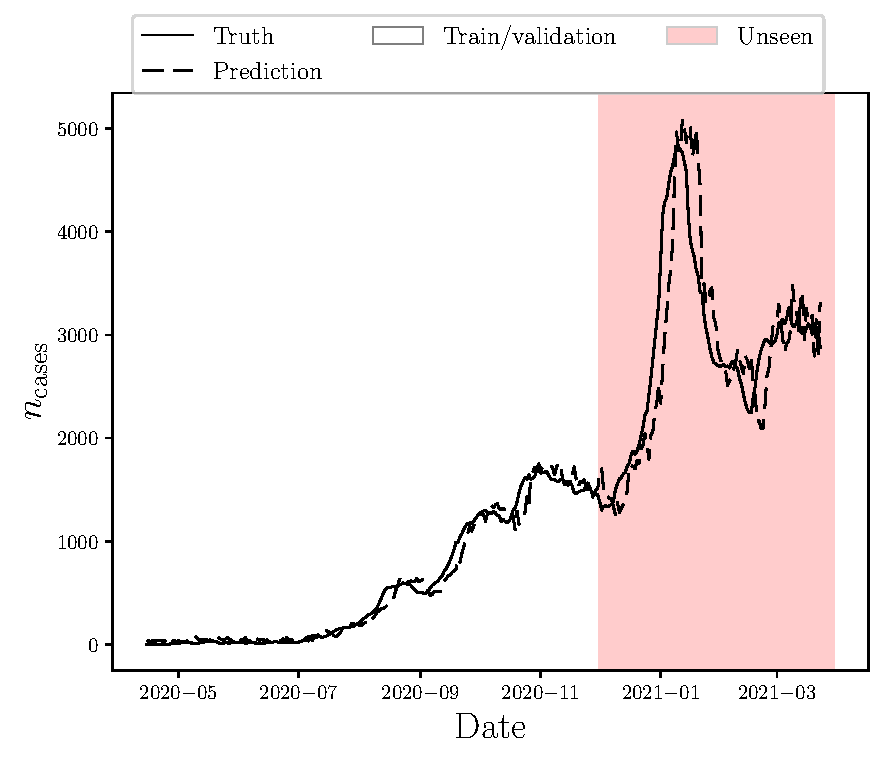
\includegraphics[width=0.5\textwidth]{predictions/model_predictions_unseen_SVR_mean_Ct_daily_cases_G12.pdf}}%
            };
		% show origin
		% \fill (0,0) circle (2pt);
	\end{tikzpicture}%
	%
	\begin{columns}[t] % The "c" option specifies centered vertical alignment while the "t" option is used for top vertical alignment
		\begin{column}{.42\textwidth} % Left column and width
			\vspace{-2.0em}
            % Column widths
            \newcommand{\ocwa}{5cm}
            \newcommand{\ocwb}{1.6cm}
            \newcommand{\ocwc}{1.6cm}
            \newcommand{\ocwd}{1.6cm}
            %
            \begin{table}[h!]
                \centering
                \footnotesize
                \renewcommand{\arraystretch}{1.5}% Wider
                \begin{tabular}{L{\ocwa}C{\ocwd}} \toprule
                    \multicolumn{1}{c}{\bf Model}               & \multicolumn{1}{c}{\bf Test error}                                \\ \toprule
                    \only<1-2>{\emphasis}{Seq2Seq}		        & \only<1>{\emphasis{0.571}}\only<2->{\bf\color{darkgreen}{0.106}}   \\
                    Long short term memory (LSTM) cell          & 0.326                                                             \\
                    feedforward neural network	                & 0.255                                                             \\
                    \only<3>{\emphasis}{Support vector machine} & \only<1-2>{0.168}\only<3>{\bf\color{darkgreen}{0.140}}            \\
                    Gradient boosting 		                    & 1.444                                                             \\
                    Linear regression 		                    & 0.160                                                             \\ \bottomrule
                \end{tabular}
            \end{table}
        \end{column}
        %
		\begin{column}{.5\textwidth} % Left column and width
		\end{column}
	
	\end{columns}
	%
	\vspace{-3em}
\end{frame}
%------------------------------------------------